\cotefile{138}
\scanpage{32}

\deleted{$\widetilde E_1$\unsure{fixe, $\alpha$|$\{\alpha,\alpha\}$}}

Soit

\[
\deleted{\widetilde C_1=\bigl\{(\zeta_1,\zeta_2,\zeta_\infty)\in\mu_3^3}
\]

\[
\begin{aligned}
\widetilde C_1&=\operatorname{Isom}(\{\underbrace{1,2,\infty}_{I}\},\mu_3)
=\bigl\{(\zeta_1,\zeta_2,\zeta_3)\in\mu_3^3\mid\\
&\hspace{17em}\zeta_1\ne\zeta_2\ne\zeta_3\ne\zeta_1\bigr\}\\[-1ex]
&\subset\deleted{\unsure{\overline{\mathbb Q}^{\,3}}}\ \text{cône projectant de }\overline C_1\subset\overline{\mathbb Q}^{\,3}
\end{aligned}\tag*{(24)}
\]

$\widetilde C_1$ a $3!=6$ éléments, et $\mu_3$ y opère diagonalement \deleted{sans point fixe} \inserted{librement (multiplication scalaire)}, le quotient $\widetilde C_1/\mu_3$ a donc deux éléments. L'application

\[
\widetilde C_1/\mu_3\longrightarrow\overline C_1
\]

\margin{\uline{NB} $\widetilde C_1/\mu_3\subset\Pi_3$ est formé des \deleted{\unsure{liens|lignes}}}

induit une bijection

\[
\widetilde C_1/\mu_3\simeq\overline C_1^{\unsure{\mathfrak S_3|\mathscr S_3}^{+}}
=\{\unsure{\sigma|\alpha|\varpi},\bar\sigma\}
\tag*{(25)}
\]

mettant en évidence l'opération de $\mathcal E$ sur $(\sigma,\bar\sigma)$, via ses opérations sur $\widetilde C_1\subset\mu_3^3=\mu_3^I$ (\uline{NB} $\mathcal E$ opère via $\mathfrak S_3\times\{\pm1\}$, avec $\Gamma\mathrel{\overset{\chi_3}{\unsure{-|\longrightarrow}}}\{\pm1\}$)

Soit alors $\widetilde C_n$ l'image inverse de $\widetilde C_1$ par l'application allant du cône projectant de $\overline C_n$, au cône projectant de $\overline C_1$, donc \deleted{c'est l'ens de $(x,y,z)$ avec \unsure{$z$}}

\[
\left\{\begin{aligned}
\overline C_n&=\{(x,y,z)\in\overline{\mathbb Q}^{\,3}\mid
\deleted{x^n+y^n+z^n=1,\ x}\inserted{(x^n,y^n,z^n)\in\widetilde C_1}\}\\
&=\{(x;y,z)\in\overline{\mathbb Q}^{\,3}\mid
x^{3n}=y^{3n}=z^{3n}=1,\ x^{\unsure{3n|n}}\ne y^n\ne z^n\ne x^n\}
\end{aligned}\right.\tag*{(26)}
\]

Noter que $\mu_{3n}$ opère diagonalement sur $\overline C_n$,

% archive sheet number: 31
\scanpage{33}

L'application

\[
\widetilde C_n\mathrel{\unsure{-|\longrightarrow}}\widetilde C_1
\]

est compatible avec

\[
\mu_{3n}\mathrel{\overset{\zeta\mapsto\zeta^n}{\rule{1.5em}{0.4pt}}}\mu_{n}
\]

et induit donc par passage au quotient

\[
\widetilde C_n/\mu_{3n}\mathrel{\rule{1.6em}{0.4pt}}\widetilde C_1/\mu_n
\]

Ceci dit, on a un diagramme comm

\diagram{\begin{tikzcd}[ampersand replacement=\&,column sep=large,row sep=large]
\text{(27)}\&\widetilde C_n/\mu_{3n}\arrow[r,no head]\arrow[d,"\wr"']\&\widetilde C_1/\mu_n\arrow[d,no head,"\wr"]\\
\& E_n(\underbrace{\{\unsure{\sigma|\alpha|\varpi},\bar\sigma\}}_{\unsure{\sigma_*|O_*|\alpha_*}})
\arrow[r,"{\substack{\text{projection}\\\text{canonique}\\\text{induite par}\\\overline C_n\mathrel{-}\overline C_1}}"']
\&E_1(\underbrace{\{\sigma,\bar\sigma\}}_{\sigma_*})
\end{tikzcd}}

Passant à la limite, on posera

\[
\widetilde C_\infty=\{(x,y,z)\in T^3\deleted{\unsure{\}|(}}= \mu_\infty^3\mid x_3\ne y_3\ne z_3\ne x_3\}
\tag*{(28)}
\]

où pour $\xi\in T$, $\unsure{\zeta_3|\xi_3}$ désigne son image dans $T/3T\simeq\mu_3$. Donc $\unsure{\xi}$

\[
\widetilde C_\infty\subset T^3\qquad\text{stable par}\quad T
\]

et on trouve un

\[
\widetilde C_\infty/T\lhook\joinrel\longrightarrow T^3/T\simeq\Pi_\infty
\tag*{(29)}
\]

\margin{$E^{21}(\unsure{\sigma_*^g|O_*^g|O_*|\alpha_*},\deleted{\unsure{a}})$}

% archive sheet number: 32
\scanpage{34}

de façon précise

\[
\begin{aligned}
\widetilde C_\infty/\mu_\infty&\simeq\text{Image inverse de }\overbrace{\overline C_1/\mu_3}^{\substack{\omega\\\unsure{\wr|\simeq}}}\subset\mu_3^3/\mu_3=\Pi_3\\
&\hspace{5em}\text{par}\quad\Pi_\infty\mathrel{\unsure{-|\longrightarrow}}\Pi_3
\end{aligned}\tag*{(30)}
\]

En \unsure{vertu|outre|termes} de la suite exacte

\[
0\mathrel{-}\Pi_\infty\mathrel{\overset{3}{\longrightarrow}}\Pi_\infty
\mathrel{\overset{p_3}{\rule{1.5em}{0.4pt}}}
\underset{\substack{\cup\\\omega}}{\Pi_3}\mathrel{-}0
\tag*{(31)}
\]

$\Pi_\infty$ opère librement sur cette \unsure{``}partie de $\Pi_\infty$, image inverse de $\omega$ par $\Pi_\infty\mathrel{-}\Pi_3$. Ceci donne les opérations de $\Pi_\infty$ sur $E(\unsure{\sigma_*|O_*|O_{\sigma}|\alpha_*})\deleted{\unsure{\{a\}}}\simeq p_3^{-1}(\omega)$, celles de $\Gamma$ et $\unsure{\mathfrak S_3|\mathscr S_3}$ \deleted{étant} induites par leurs opérations sur $\Pi_\infty$ ....

\uline{NB} Sur $\Pi_3$ $\deleted{\unsure{E\times|\mathcal E\times}}\mathfrak S_3\times\Gamma$ opère via $\mathfrak S_3\times\overbrace{\{\pm1\}}^{\substack{\text{opère par}\\\text{homothéties}\\\text{sur }\Pi_3}}$, ($\Gamma\mathrel{\overset{\chi_3}{\rule{1.5em}{0.4pt}}}\{\pm1\}$). Considérons $\mathfrak S_3^+\inserted{\simeq\mathbb Z/3\mathbb Z}$ opérant sur $\Pi_3$ ($\simeq\mathbb F_3^2$), alors on sait qu'il doit y avoir une droite invariante -- \deleted{et les} en fait elle est unique -- et $\omega$ est formé des deux éléments non nuls de cette droite ....

% archive sheet number: 33
\scanpage{35}

(1.8) Considérons enfin les pts fixes

\[
\deleted{\beta_0}\inserted{\alpha'(0)}=2,\qquad
\deleted{\beta_1}\inserted{\alpha'(1)}=-1,\qquad
\deleted{\beta_\infty}\inserted{\alpha'(\infty)}=\tfrac12
\tag*{(32)}
\]

\figure{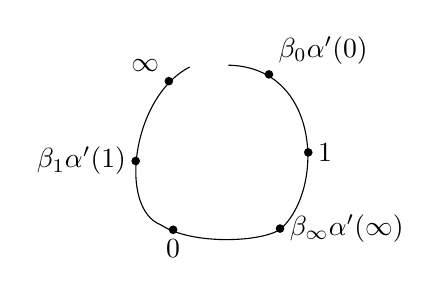
\begin{tikzpicture}[scale=.78]
\draw (0.62,2.75) .. controls (-.32,2.27) and (-.55,.45) .. (.15,.18) .. controls (.67,-.16) and (1.83,-.10) .. (2.11,.12) .. controls (2.82,.78) and (2.74,2.75) .. (1.25,2.78);
\fill (.28,2.52) circle(2pt) node[above left] {$\infty$};
\fill (1.91,2.63) circle(2pt) node[above right] {$\deleted{\beta_0}\alpha'(0)$};
\fill (2.55,1.36) circle(2pt) node[right] {$1$};
\fill (2.09,.12) circle(2pt) node[right] {$\deleted{\beta_\infty}\alpha'(\infty)$};
\fill (.35,.10) circle(2pt) node[below] {$0$};
\fill (-.26,1.22) circle(2pt) node[left] {$\deleted{\beta_1}\alpha'(1)$};
\end{tikzpicture}}

qui sont les pts fixes, autres que $0,1,\infty$ resp., des transpositions $\tau_0,\tau_1,\tau_\infty\in\unsure{\mathfrak S_3|\mathscr S_3}$. Soit

\[
\boxed{\deleted{\unsure{\beta'_*}}\alpha'_*=\{\deleted{\beta_0}\alpha'(0),\deleted{\beta_1}\alpha'(1),\deleted{\beta_2}\alpha'(2)\}.}
\tag*{(33)}
\]

On veut déterminer $E(\deleted{\beta'_*}\alpha'_*)\inserted{=\coprod_{i\in I}E(\deleted{\beta_i}\alpha'(i))}$ comme $\mathcal E$-ensemble.

On trouve

\[
\left\{\begin{aligned}
E_n(\deleted{\beta_i}\alpha'(i))&\simeq\{(\unsure{\zeta|\xi}_j)\in\overline{\mathbb Q}^{I\setminus\{i\}}\mid \zeta_j^n=-\tfrac12\quad\forall j\in I\setminus\{i\}\}\\
&\simeq K_n(-\tfrac12)^{I\setminus\{i\}}\\
E(\deleted{\beta_i}\alpha'(i))&\simeq K(-\tfrac12)^{I\setminus\{i\}}
\end{aligned}\right.\tag*{(34)}
\]

où $\forall\,\unsure{\zeta_0|\xi_0|g}\in\overline{\mathbb Q}$, on pose

\[
\left\{\begin{aligned}
K_n(\zeta)&=\{\zeta\in\overline{\mathbb Q}\mid\zeta^n=\zeta_0\}\\
K_\infty(\zeta)&=K(\zeta)=\varprojlim_n K_n(\zeta)
\end{aligned}\right.\tag*{(35)}
\]

$K_\infty(\zeta)$ étant un torseur sous $T=\mu_\infty$, sur lequel $\Gamma$ opère (donc un $\deleted{\unsure{(T,|\mathrm{Ext}}}(\mu_\infty,\Gamma)$-torseur ...)

Ici on aura, en vertu des \unsure{rel. can.|iso. can.}

\[
K(\zeta\unsure{\zeta'|g'} )\deleted{\unsure{\circ}}\simeq K(\zeta)\wedge_{\unsure{\Pi_\infty|T}}K(\zeta')
\]

\[
K(-\tfrac12)\simeq K(-1)\wedge_T K(\tfrac12)\simeq K(-1)\wedge_T K(2)^{-1}
\tag*{(36)}
\]

\[
\underset{\wr\,p_2^{-1}(\{-1\})}{K(-1)}\lhook\joinrel\longrightarrow\deleted{\unsure{E_0}}T,\qquad
(1\mathrel{-}T\mathrel{\overset{2}{-}}T\mathrel{\overset{p_2}{-}}\mu_2\longrightarrow\unsure{1|0})
\tag*{(37)}
\]

% archive sheet number: 34
\scanpage{36}

Soit

\[
\unsure{\mathcal A^{*}|\mathcal A^{\times}|A}=\deleted{\operatorname{Aff}}\operatorname{Aut}(T,K(\tfrac12))\deleted{=\operatorname{Aff}\unsure{(}}
\tag*{(38)}
\]

donc

\[
1\longrightarrow\deleted{\unsure{\mu_\infty}}T\mathrel{\unsure{-|\longrightarrow}}\mathcal A\longrightarrow
\underset{\substack{\wr\\\operatorname{Aut}(T)}}{\widehat{\mathbb Z}^{\times}}\mathrel{-}1.
\tag*{(39)}
\]

\deleted{Les \inserted{groupes $\mu_n,\mu_\infty=T$,} ensembles $\Pi_n,\Pi_\infty$, et les ensembles $\underline E(I),E(I)$ \unsure{soit} \unsure{d'où un hom} \inserted{$\underline E(\alpha_*),E(\alpha_*)$}}

\[
\deleted{\Gamma\longrightarrow\mathcal A}
\]

$\mathcal A$ opère sur $\Pi_n,\Pi_\infty\inserted{=T^3/T}$ par l'intermédiaire de $\widehat{\mathbb Z}^{*}$, (par homothéties \unsure{adiques|adéquates} \unsure{..|...}) et le groupe

\[
\widetilde{\mathcal E}=(\unsure{\mathfrak S_3|\mathscr S_3}\times\mathcal A)\underset{1/2}{\cdot}\Pi_\infty
\]

% slanted
\margin{$\alpha(0)=0$\\ $\alpha(1)=1$\\ $\alpha(\infty)=\infty$\\ $\alpha(*)=\{\alpha(0),\alpha(1),\alpha(\infty)\}$}

opère \inserted{de façon évidente} sur les ensembles $\underline E_n(\alpha\unsure{(*)|{}_*}),E(\alpha_*))$ $\underline E(\unsure{\sigma|\alpha|\varpi}_*),E(\sigma_*),\underline E(\deleted{\beta_*}\alpha'_*),E(\deleted{\beta_*}\alpha'_*)$, -- en fait sur les quatre premiers il opère via le quotient $\deleted{\widetilde{\mathcal E}/T\simeq}\unsure{\widehat{\mathbb Z}}$

\[
\widetilde{\mathcal E}/T\simeq(\mathfrak S_3\times\widehat{\mathbb Z}^{\times})\underset{1/2}{\cdot}\Pi_\infty .
\]

D'autre part, on a

\[
\Gamma\mathrel{\rule{3em}{0.4pt}}\mathcal A
\tag*{(40)}
\]

hom dont l'image \inserted{$\Gamma'$} est d'indice fini (est-on $=$ surjectif) $\Gamma'$ est le groupe de Galois de la sous-extension de $\unsure{\overline{\mathbb Q}|\mathbb Q}/\unsure{\overline{\mathbb Q}|\mathbb Q}$ engendrée par toutes les racines $n$-ièmes de $\tfrac12$,

\margin{?}

% archive sheet number: 35
\scanpage{37}

pour $n$ variable. Ceci dit, on a un hom évident

\[
\mathcal E=(\unsure{\mathfrak S_3|\mathscr S_3}\times\Gamma)\underset{1/2}{\cdot}\Pi_\infty\longrightarrow
\widetilde{\mathcal E}=(\mathfrak S_3\times\mathcal A)\underset{1/2}{\cdot}\Pi_\infty
\tag*{(41)}
\]

déduit de (40), et les opérations de $\mathcal E$, \unsure{sur|en} les ens. précédents se font \uline{à travers} $\widetilde{\mathcal E}$ ....

(1.9) Les développements précédents n'utilisaient pas que \deleted{$\mathbb Q$}la clôture alg. \inserted{envisagée} $\overline{\mathbb Q}$ de $\overline{\mathbb Q}$ était plongée dans $\mathbb C$ -- ils marcheraient $=$ en remplaçant $\mathbb Q$ par n'importe quel corps premier, à condition de se borner à des $n$ premiers à la car. ($\overline C_\infty$ est alors le revêtement universel abélien \uline{modéré} de $(\overline C_1,I)$ ...). Il faut l'utiliser, pour faire le lien avec les cartes $3$-pondérées finies abéliennes, et le groupe cartographique.

On va d'abord \unsure{pointer|ponctuer|trivialiser} $\overline C_\infty$ au dessus de $\unsure{\sigma|\alpha|\varpi}=-\bar j\in\omega=\{\sigma,\bar\sigma\}$, pour pouvoir l'identifier au rev. universel profini \deleted{pointé} \uline{sur $\sigma$}.

% archive sheet number: 36
\scanpage{38}

Rappelons

\[
\underset{\substack{\Vert\\p_3^{-1}(\alpha)}}{E(\unsure{\sigma_*|\alpha_*|\alpha})}\subset\Pi_\infty\xrightarrow{p_3}\Pi_3
\tag*{(42)}
\]

\[
\underset{\deleted{\unsure{-\bar j}}}{\unsure{\sigma|\alpha}}
=(\bar j,\deleted{\bar{\vphantom j}}j,1)\bmod\mu_3
=\underset{\substack{\rotatebox{-90}{$\in$}\\\Pi_3}}{\{(\bar j,\deleted{\bar{\vphantom j}}j,1),(\deleted{\bar{\vphantom j}}j,1,\bar j),(1,\bar j,\deleted{\bar{\vphantom j}}j)\}}
\]

\deleted{Posons} Nous \deleted{prendrons} utiliserons

\[
(\qquad j=\exp\tfrac{2i\pi}{3},\qquad \bar j=\exp-\tfrac{2i\pi}{3}
\]

et poserons

\[
\zeta_n=\exp\tfrac{2i\pi}{3n}
\tag*{(43)}
\]

et

\[
\left\{\begin{aligned}
\deleted{\unsure{\alpha_n\text{ soit }\zeta_n}}\ \sigma_n
&=(\bar\zeta_n,\deleted{\bar{\vphantom\zeta}}\zeta_n\deleted{j},1\deleted{\unsure{\zeta}})
&&\left\{\begin{aligned}
&\text{considéré soit comme un}\\[-.3ex]
&\text{élément de }\overline C_n\text{ au dessus de }\sigma=-j\\
&\deleted{\bmod\mu_n\text{ dans}}\\
&\text{soit comme élément de }\mu_{3n}^{\,3}\bmod\mu_{\unsure{3n|3}}\\
&\deleted{\unsure{\text{définisse}}}\\[-.3ex]
&=\Pi_{3n}
\end{aligned}\right.\\
\sigma_\infty&=\begin{aligned}
&\deleted{\unsure{(\zeta_\infty,\bar\zeta_\infty,1)}}\\
&(\bar\zeta_\infty,\zeta_\infty,1)
\end{aligned}
&&\left\{\begin{aligned}
&\text{considéré soit comme pts de}\\
&\overline C_\infty\text{ au dessus de }\alpha=-j\\
&\text{soit comme él. de }\mu_\infty^{\,3}\bmod\mu_\infty\\
&=\Pi_\infty
\end{aligned}\right.
\end{aligned}\right.
\]

où

\[
\zeta_\infty=(\zeta_n)\in T
\tag*{(\deleted{\unsure{4}}44)}
\]

est la base canonique de $T$, donnée par l'exponentielle complexe, permettant donc de définir un \unsure{isom. can|iso. can.}

\[
\widehat{\mathbb Z}\mathrel{\overset{\varphi}{\simeq}}T .
\tag*{(45)}
\]

% archive sheet number: 37
\scanpage{39}

Maintenant on déduit donc des isom

\[
\left\{\begin{aligned}
\Pi_\infty&\simeq\widehat{\mathbb Z}^{3}/\widehat{\mathbb Z}\\
&\deleted{\unsure{\mathcal E|E}\simeq(\unsure{\mathfrak S_3|\mathscr S_3}\times\widehat{\mathbb Z}^{\unsure{3|\times|*}}/\widehat{\mathbb Z}}\\
\deleted{\unsure{\mathcal A}}\mathcal E&\simeq(\underbrace{\mathfrak S_3\times\Gamma}_{\substack{\text{opère via}\\\text{permutation des}\\\text{facteurs et}\\\text{via homothétie}\\\text{par }\chi:\Gamma\longrightarrow\widehat{\mathbb Z}^{\times}}})\underset{1/2}{\cdot}(\widehat{\mathbb Z}^{3}/\widehat{\mathbb Z})
\end{aligned}\right.\tag*{(46)}
\]

\inserted{\tikz[baseline=(fin.base)]{\node[ellipse,draw,inner sep=4pt] (fin) {$\Pi_n\simeq(\mathbb Z_{/n})^3/\mathbb Z_n$};\draw[->] (fin.east) to[out=15,in=-90] ++(1.2,1.3);}}

\[
\unsure{\dot\sigma_\infty|\sigma_\infty|o_\infty|\alpha_\infty}\simeq(-1,+1,0)\bmod\widehat{\mathbb Z}\qquad\text{d'où}
\tag*{(47)}
\]

\[
o'_\infty=\overline{\unsure{\sigma_\infty|\sigma'_\infty|\alpha_\infty}}=(1,-1,0)\bmod\widehat{\mathbb Z}
\tag*{(47$'$)}
\]

Considérons les éléments

\[
\left\{\begin{aligned}
&\rho_0,\rho_1,\rho_\infty\in\Pi_\infty\\
&\rho_0=(1,0,0)\quad\bmod\widehat{\mathbb Z}\\
&\rho_1=(0,1,0)\quad\rule{2.4em}{0.4pt}\\
&\rho_\infty=(0,0,1)\quad\rule{2.4em}{0.4pt}
\end{aligned}\right.\tag*{(48)}
\]

de sorte que

\[
\rho_0\,\rho_1\,\rho_\infty=1
\tag*{(49)}
\]

$\big\Vert$ Ce sont ces éléments qui donnent l'isom de $\widehat{\unsure{\mathrm{Gr}|\mathrm G|\Gamma}}_2^+$ avec $\Pi_\infty$.

% archive sheet number: 38
\scanpage{40}

\deleted{Il reste à définir le}

Il faut expliciter $K(2)$, \deleted{\unsure{comme}} en choisissant une origine

\[
\theta_\infty=(\underbrace{\sqrt[n]{2}}_{\theta_n})_{n\in\mathbb N^*}
\tag*{(\unsure{56|50})}
\]

donc $K(2)$ est identifié à $T$ donc à $\widehat{\mathbb Z}$, et

\[
\deleted{\mathcal A}\qquad\mathcal A\simeq\operatorname{Aff}(1,\widehat{\mathbb Z})\simeq\widehat{\mathbb Z}^{\times}\underset{1/2}{\cdot}\widehat{\mathbb Z}
\tag*{(51)}
\]

opérant sur $K(2)\simeq\widehat{\mathbb Z}$ de façon tautologique

\[
(\underset{\substack{\rotatebox{-90}{$\in$}\\\widehat{\mathbb Z}^{\times}}}{a},
\underset{\substack{\rotatebox{-90}{$\in$}\\\widehat{\mathbb Z}}}{b})(\underset{K(2)}{x})=ax+b
\tag*{(52)}
\]

On a donc

\[
K(\tfrac12)\simeq\widehat{\mathbb Z}
\tag*{(53)}
\]

mais \unsure{opération|opérations}

\[
(\underset{\substack{\rotatebox{-90}{$\in$}\\\widehat{\mathbb Z}^{\times}}}{a},
\underset{\substack{\rotatebox{-90}{$\in$}\\\mathbb Z}}{b})(\underset{K(1/2)}{x})=ax-b
\tag*{(54)}
\]

Ceci permet d'expliciter entièrement $E(\beta_*)$ en plus de $E(\omega)$ ...

Il reste \inserted{enfin} à expliciter les hom de transport parallèle

\diagram{\begin{tikzcd}[ampersand replacement=\&,column sep=small,row sep=small]
\& E_0\\
E(\alpha)\arrow[ur]\arrow[r,no head]\arrow[dr]\&E_1\\
\&E_\infty
\end{tikzcd}}

et

\diagram{\begin{tikzcd}[ampersand replacement=\&,column sep=small,row sep=small]
\& E'_0=E_2\\
E(\alpha)\arrow[ur,"\sim"]\arrow[r,no head,"\sim"]\arrow[dr,"\sim"']\&E'_1=E_{-1}\\
\& E'_\infty\simeq E_{1/2}
\end{tikzcd}}

\diagram{\begin{tikzcd}[ampersand replacement=\&,column sep=small,row sep=0pt]
\text{[et}\&E'_0\arrow[r,no head]\arrow[dr,no head]\&E_1\&E'_1\arrow[r,no head]\arrow[dr,no head]\& E_\infty\& E'_\infty\arrow[r,no head]\arrow[dr,no head]\&E_0\\
\&\&E_\infty\&\&\deleted{\unsure{E_1}}E_0\&\&E_1\ \text{]}
\end{tikzcd}}

\margin{?}

d'où on déduit les \unsure{6} hom correspondants de $E(\bar\alpha)$ en conjuguant par la conjugaison complexe. Comme ce sont des hom

% archive sheet number: 39
\scanpage{41}

compatibles avec l'action de $\Pi_\infty$ et de $\unsure{\mathfrak S_3|\mathscr S_3}\deleted{\unsure{\Gamma}}\times\underline{\{1,\tau\}}$ ($\tau\inserted{\in\Gamma}$ étant la conjugaison complexe) il suffit pour déterminer ces $18$ flèches, de déterminer deux d'entre elles, \deleted{telles que} \inserted{p. ex}

\[
E(\underset{\substack{\Vert\\\alpha_1}}{\alpha})\longrightarrow
\underset{\substack{\Vert\\E_{1/2}}}{E'_\infty}\longrightarrow E_0
\]

[NB $E(\alpha)\mathrel{\unsure{-|\longrightarrow}}E_0$ est le composé] et $=$ de connaître \inserted{les} images dans $E_0,E_1$ de l'élément marqué $\unsure{\sigma_\infty|\alpha_\infty}$ de $E(\sigma)$, [d'où élément marqué $\deleted{\beta}\alpha'_\infty(i)\in E'_i=\deleted{\unsure{/|,}}E(\alpha'(i))$, et $\deleted{E}\alpha_\infty(i)\in E_i=E(\alpha(i))$, $\forall i\in\{0,1,\infty\}$].

On trouve

\[
\begin{aligned}
\alpha'_n(\infty)&=\left(\sqrt[n]{\tfrac12}\exp\tfrac{-\pi i}{n},\sqrt[n]{\tfrac12}\exp\tfrac{+\pi i}{n},1\right)\\
&=(\deleted{\unsure{\varphi}}\theta_n^{-1}\bar\zeta_n,\theta_n^{-1}\zeta_n,1)\\
\deleted{\alpha'_\infty(\infty)}&\deleted{=}\\[-.6ex]
\alpha'_\infty(\infty)&=(\theta_\infty\wedge\bar\zeta_{\unsure{n|\infty}},\theta_\infty\wedge\zeta_\infty,1)
\end{aligned}
\]

% archive sheet number: 40
\scanpage{42}

\[
I\in\operatorname{Ob}\operatorname{Ens}_3
\]

\[
\left.\begin{aligned}
\Pi(\deleted{\unsure{*}}I)&=\widehat{\mathbb Z}^{I}/\widehat{\mathbb Z}\\
\Pi_n(I)&=\mathbb Z_{/n}^{I}/\mathbb Z_{/n}
\end{aligned}\right|
\]

\diagram{\begin{tikzcd}[ampersand replacement=\&,column sep=small,row sep=tiny]
\&\text{\unsure{permut.|structurel}}\& \text{hom.}\\
\unsure{\mathfrak S_I|\mathscr S_I}\arrow[ur]\&{}\times\widehat{\mathbb Z}^{\times}\arrow[ur,no head]\&\text{y opère}
\end{tikzcd}}

\[
\unsure{\mathcal E''|E''|\mathcal E''_1}(I)\simeq(\mathfrak S_I\times\widehat{\mathbb Z}^{\times})\underset{1/2}{\cdot}\unsure{\dot\Pi|\Pi|\pi}(I)
\]

\[
E(I,\underset{\substack{\rotatebox{-90}{$\in$}\\I}}{i})\simeq\widehat{\mathbb Z}\wedge_{(\pm1)}(I\setminus\{i\})
\]

\[
E(I;I)\simeq\coprod_{i\unsure{\in|\notin}I}E(I,i)
\]

\[
\deleted{\unsure{E_*}}\qquad\omega\simeq\operatorname{Or}(I)\wedge\{j,\bar j\}\simeq\operatorname{Or}(I)\subset\Pi_3=
\underset{\substack{\Vert\\\mathbb F_3^{I}/\mathbb F_3}}{(\mathbb Z_{/3})^{I}/\mathbb Z_{/3}}
\]

\diagram{\begin{tikzcd}[ampersand replacement=\&,column sep=tiny,row sep=small]
\& E(I,\omega)=p_3^{-1}(\omega)\subset\Pi_\infty(I)\arrow[dl,"{\deleted{\unsure{\alpha_\infty(\omega)}}}"']\\
E(I,i)\&
\end{tikzcd}}

\[
0\mathrel{-}\Pi_\infty(I)\mathrel{\unsure{-|\longrightarrow}}\Pi_\infty(I)\longrightarrow\underset{\substack{\cup\\\omega}}{\Pi_3(I)}\mathrel{-}0
\]

% archive sheet number: 41
\scanpage{43}

% letterhead
U N I V E R S I T E\\
DES SCIENCES ET TECHNIQUES\\
DU LANGUEDOC\\
\rule{3em}{0.4pt}

Montpellier, le 15 Juin 1978\\

MR/FP\\
\uline{Diffusion}: Liste A\\
n\textsuperscript{o} 3762

% printed form
\uline{AVIS DE SOUTENANCE D'UNE THESE DE DOCTORAT}\\
\uline{D'UNIVERSITE}

\uline{Nom et Prénom du candidat} : GOUSSOPOULOS Jean

\uline{Titre de la thèse} : Etude de la croissance relative postnatale chez le poulet. Principaux tissus et organes, muscles et os individuels. Influence de l'hypophysectomie.

\uline{Date, heure et lieu de soutenance prévus} : 5 Juillet 1978 à 9 heures - U.S.T.L. MONTPELLIER - ENSAM. Laboratoire Zootechnie.

\uline{Nom du Directeur de thèse} : L. DAUZIER

\uline{Désignation du laboratoire où la thèse est préparée} : Station de Physiologie Animale - INRA - MONTPELLIER

\uline{Analyse de l'ouvrage} : Etude descriptive par l'utilisation d'allométrie, de la croissance pondérale relative chez le poulet : principaux tissus et organes ; os et muscles individuels. Mise en évidence de gradients de croissance et de différences de développement selon le sexe. Effets de l'hypophysectomie, dont l'influence est surtout nette au niveau du muscle et du tissus gras.

\uline{Durée approximative des recherches ayant abouti à la thèse} : 5 ans

\uline{Composition du jury proposé} : \quad L. DAUZIER, Président\\
\hspace*{12em}C. THIBAULT\\
\hspace*{12em}J.D. BAYLE\\
\hspace*{12em}M. BENEVENT

Le Secrétaire Général,\\

\handwritten{\unsure{E. Siau}}\\

\uline{E. SIAU.}

% archive sheet number: 42
\scanpage{44}

Genre de la courbe de Fermat $C_n$ (qui est une courbe \deleted{\unsure{projective}}\inserted{plane} lisse de degré $n$)

\[
g_n=\frac{(n-1)(n-2)}{2}
\]

le genre est $0$ \unsure{sss|ssi} $n=1,2$, il est $1$ sss $n=3$. Pour $n=4$ il est $3$, pour $n=6$ il est $10$, pour $n=12$ il est $55$ .....

\centerline{\rule{4em}{0.4pt}}
Considérons le cas $n=2$

\[
C_2:\quad x^2+y^2+z^2=0
\]

comme carte triangulée pondérée elle est formée de $4.2=8$ triangles, chaque type de sommet intervient $2$ fois, avec degré $4$ \inserted{($=2.2$)} \unsure{pour des gens au courant.|pour degré en un vert.|pour les gens au courant.} Sauf erreur, c'est l'\uline{\unsure{octoèdre|octaèdre}} \inserted{sphérique}, dont le groupe des automorphismes orientés est bien \inserted{$\simeq$}$\unsure{\mathfrak S_4|\mathscr S_4}$ d'ordre $24$, et peut s'écrire comme produit $1/2$ direct de $\mathfrak S_3$ par $(\mathbb Z_2)^2$ !

\figure{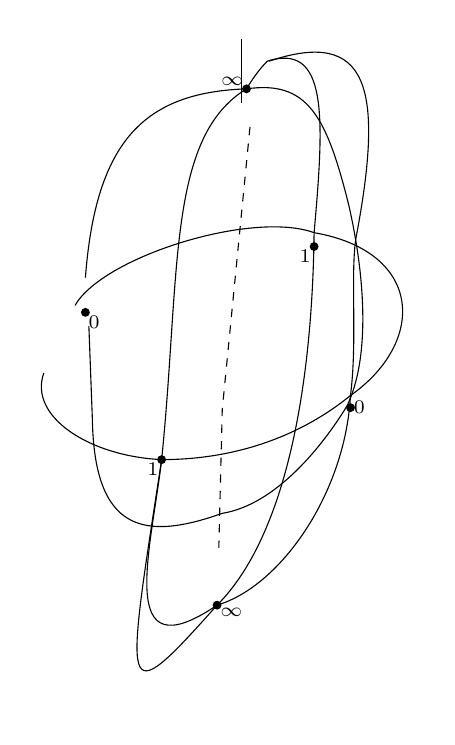
\begin{tikzpicture}[x=.022cm,y=-.022cm,every node/.style={font=\scriptsize,inner sep=1pt}]
\draw (120,5)--(120,42);
\draw (30,143) .. controls (36,64) and (64,36) .. (123,34) .. controls (158,29) and (169,49) .. (182,101) .. controls (192,145) and (194,190) .. (181,217) .. controls (167,240) and (140,274) .. (109,279) .. controls (64,295) and (35,290) .. (34,224) -- (32,171);
\draw (24,159) .. controls (40,131) and (126,104) .. (162,117) .. controls (225,128) and (227,180) .. (183,211) .. controls (156,233) and (119,248) .. (74,248) .. controls (32,246) and (-3,223) .. (6,198);
\draw (123,34) .. controls (77,62) and (85,140) .. (74,248) .. controls (68,300) and (47,372) .. (106,332) .. controls (146,292) and (161,205) .. (162,117) .. controls (168,50) and (170,7) .. (135,18) .. controls (130,23) and (126,29) .. (123,34);
\draw (136,18) .. controls (193,-1) and (203,32) .. (186,121) .. controls (183,143) and (187,180) .. (183,211) .. controls (180,267) and (143,321) .. (106,332) .. controls (49,396) and (53,386) .. (74,248);
\draw[dashed,thin] (125,56)--(109,219)--(107,299);
\fill (123,34) circle(1.6pt) node[above left] {$\infty$};
\fill (30,163) circle(1.6pt) node[below right] {$0$};
\fill (162,125) circle(1.6pt) node[below left] {$1$};
\fill (183,218) circle(1.6pt) node[right] {$0$};
\fill (74,248) circle(1.6pt) node[below left] {$1$};
\fill (106,332) circle(1.6pt) node[below right] {$\infty$};
\end{tikzpicture}}

Divisant par les trois ss-gpes $\mathbb F_2$ de $\Pi_2\simeq\mu_2^3/\mu_2$, on trouve les \inserted{$3$} revêtements d'ordre $2$ de $C_1\simeq\mathbb P^1_{\mathbb Q}$ qui correspondent au \deleted{dièdre}\inserted{monoèdre} \deleted{\unsure{pointés}} (autodual) et à ses transformés par $\mathfrak S_3$

\margin{\uline{NB} L'octaèdre est subdivision barycentrique du bi-èdre (qui est autodual) et a le type de ramification}

\figure{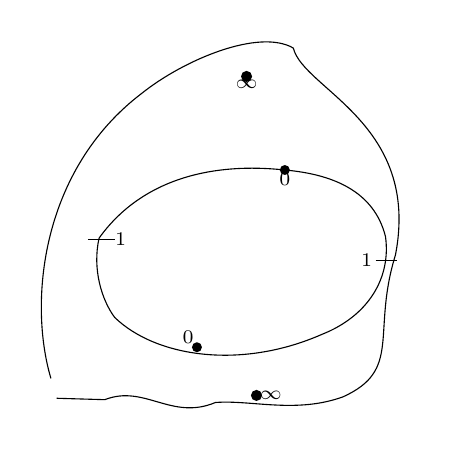
\begin{tikzpicture}[x=.018cm,y=-.018cm,every node/.style={font=\scriptsize,inner sep=1pt}]
\draw (3,238) .. controls (-13,184) and (-4,91) .. (67,37) .. controls (97,13) and (150,-9) .. (174,5) .. controls (181,34) and (264,58) .. (246,151) .. controls (229,206) and (251,232) .. (209,251) .. controls (176,263) and (144,253) .. (119,255) .. controls (88,268) and (69,242) .. (41,253) -- (7,252);
\draw (37,139) .. controls (65,100) and (112,85) .. (168,91) .. controls (202,94) and (231,106) .. (239,138) .. controls (243,167) and (227,194) .. (194,207) .. controls (137,232) and (77,223) .. (48,195) .. controls (39,183) and (32,161) .. (37,139);
\draw (29,140)--(48,140) (232,155)--(247,155);
\node[right] at (46,140) {$1$};\node[left] at (232,155) {$1$};
\fill (141,25) circle(2pt) node[below] {$\infty$};
\fill (168,91) circle(1.8pt) node[below] {$0$};
\fill (106,216) circle(1.8pt) node[above left] {$0$};
\fill (148,250) circle(2pt) node[right] {$\infty$};
\end{tikzpicture}}

\[
\begin{array}{ccc}2&2&2\\2&2&2\end{array}
\]

\margin{(cas particulier de celle du \unsure{$n$-èdre|$N$-èdre|dièdre} $\begin{array}{ccc}n\left\{\begin{smallmatrix}2\\\vdots\\2\end{smallmatrix}\right.&n\left\{\begin{smallmatrix}2\\\vdots\\2\end{smallmatrix}\right.&\begin{smallmatrix}n\\n\end{smallmatrix}\end{array}$, pour $n=2$), ce qui \uline{\unsure{caractérise|confirme}}, on le voit de suite, le rev. abélien universel annulé par $2$ ...}

% archive sheet number: 43
\scanpage{45}

% letterhead
U N I V E R S I T E\\
DES SCIENCES ET TECHNIQUES\\
\uline{DU LANGUEDOC}\\
JFR/MD\\

Montpellier, le \textit{22 Juin 1978}\\

LE DIRECTEUR DE L'U. E. R. III\\
à\\
Mesdames et Messieurs les Membres\\
des Jurys des examens de l'U.E.R. III\\

\deleted{Madame, Monsieur,\\

Le Conseil de l'U.E.R. III se permet de vous rappeler qu'une réforme des maîtrises spécialisées est en cours, et que tous les dossiers d'habilitation ou de reconduction devront parvenir au Ministère avant le 31 janvier 1979.

Pour faciliter sa tâche il vous serait reconnaissant de bien vouloir lui indiquer si vous désirez que la maîtrise où vous enseignez soit reconduite ou si vous souhaitez la modifier en tout ou partie.

Il a pensé que les jurys des différents certificats étaient les plus propres à diffuser cette lettre auprès des enseignants qui s'estiment concernés. Il espère qu'ils voudront bien examiner attentivement ce problème.

Il accueillera toute suggestion dont vous pourriez lui faire part avant le 15 octobre 1978.

Il compte sur votre aide et vous prie de croire à tout son dévouement.

Le Directeur de l'U.E.R. III,\\

\handwritten{\uline{\unsure{Jean Regnier|Jean Régnier}}}\\

\uline{J.F. REGNIER}\\

\textit{\uline{N.B.} : Cette lettre a été transmise pour information aux Directeurs d'U.E.R. et aux Membres du Conseil de l'U.E.R. III.}}

% archive sheet number: 44
